\documentclass[10pt,twocolumn]{article}
\usepackage{fullpage,times,graphicx}

%opening

\begin{document}

\section*{High-Level GPGPU Programming with Parakeet}
We present Parakeet, an intelligent runtime library and JIT compiler which enables high-level languages such as Python's NumPy to take advantage of GPU acceleration -- all while requiring no changes to existing code.

while dynamically translating and executing array-oriented subsets of user programs on NVIDIA GPUs.

into a typed intermediate language and performs optimizations that eliminate costly abstractions and increase computational density. Parakeet then executes its intermediate representation by quickly synthesizing and executing data parallel GPU programs. Parakeet's runtime transparently handles data movement, GPU memory space selection, data layout, as well as garbage collection. Parakeet is attached as a library to the source language's interpreter, allowing all of the source language's standard features and tools to be used.

% Enable programmers to write GPGPU programs in productivity language
GPUs are able to achieve impressive performance in certain cases because they have been highly specialized for data parallel workloads.  Array programming languages are thus well suited for high level GPU programming due to their idiomatic preference for data parallel array operations instead of explicit loops (``collection-oriented''~\cite{Sip91} programming). We observe that many of the above projects are structured around the use of data parallel array operators such as map and reduce.

% Heart of Parakeet - an interpreter for our high level IL w/ array ops
In this paper, we present Parakeet, an intelligent runtime for executing high level array programs on GPUs. Parakeet is neither a new programming language, nor is it tied to any specific language. The Parakeet library is designed to accelerate the array oriented constructs of existing dynamic languages. A key objective is to harness the elegance and parallelizability of functional array operators while sacrificing as little programmer convenience as possible.  Specifically, Parakeet supports the use of array language semantics such as scalar promotion as well as a restricted use of mutable state.

% Q front-end, agnosticism
We have implemented our first Parakeet front end for Q~\cite{Borr08}, a descendant of APL that is widely used in financial computing. Q is particularly amenable to GPU acceleration by Parakeet as its use of array operators is very extensive -- its idiomatic style makes sparser use of loops than even Matlab~\cite{Moler80} or Python's NumPy extensions~\cite{Oliphant07}. We are also developing a front end for NumPy.

\begin{figure}[h!]
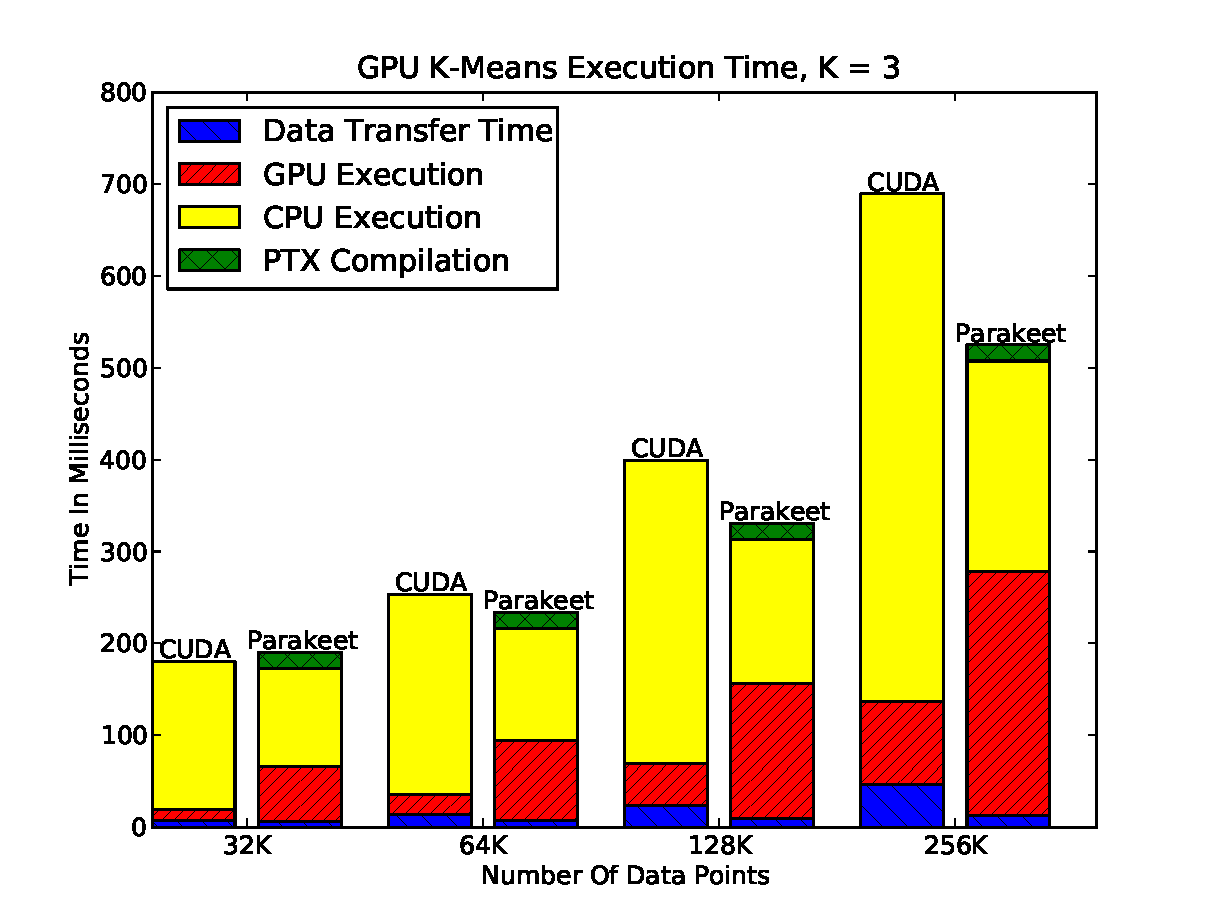
\includegraphics[scale=0.45]{KMGPU.pdf}
\label{BSGPU}
\end{figure}

\end{document}
